\chapter{جمع‌بندي و نتيجه‌گيري و پیشنهادات}
\section{نتایج}
%%%%%%%%%%%%%%%%%%%%%%%%%%%%%%%%%%%%%%%%%%%
\subsection{نتایج شبیه‌سازی الگوریتم درخت جستجوی تصادفی}
در ابتدا نتایج حاصل از شبیه‌سازی توسط پایتون قرار داده‌ شده‌است. همانطور که در شکل
\ref{نتیجه شبیه‌سازی RRT}
قابل مشاهده است، یک محیط با ابعاد مشخص و تعداد موانع مشخص طراحی و سپس با تعیین نقطه شروع و پایان برای ربات، با استفاده از الگوریتم پیشنهادی ربات توانسته است مسیر خود را بدون برخورد با موانع بیابد.
\begin{figure}[H]
	\centering
	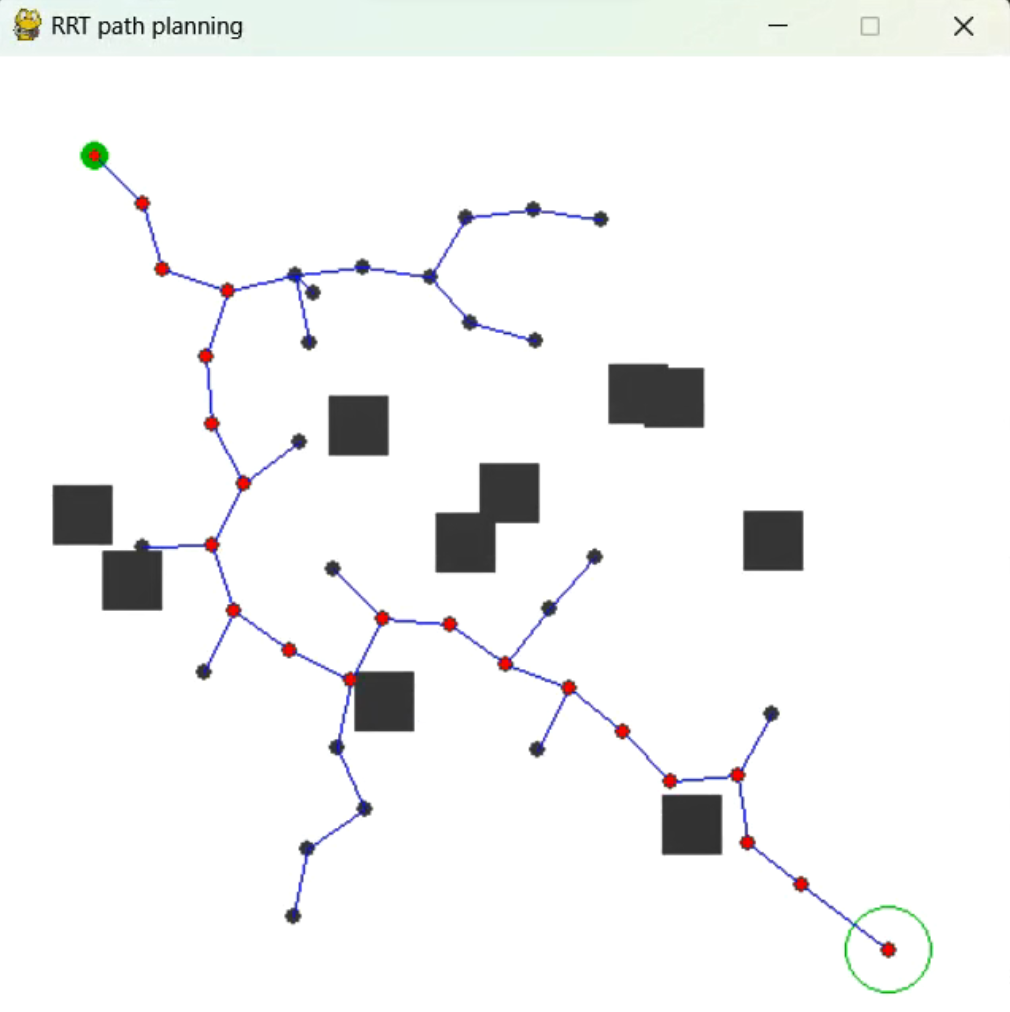
\includegraphics[width=0.7\textwidth]{./images/Chapter2/ConvexResult}	
	\caption[شبیه سازی الگوریتم \lr{RRT}]{شبیه سازی الگوریتم \lr{RRT}}
	\label{نتیجه شبیه‌سازی RRT}
\end{figure}
\noindent
\unskip
\newpage

\subsection{نتیجه تشخیص مانع}

\begin{figure}[H]
	\centering
	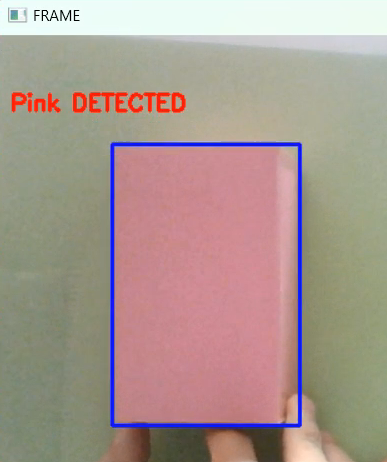
\includegraphics[width=0.6\textwidth]{./images/Chapter2/PinkDetected}	
	\caption[مانع مکعب مستطیل با رنگ صورتی]{مانع مکعب مستطیل با رنگ صورتی}
	\label{PinkDetected}
\end{figure}
\noindent
\unskip

\newpage
\subsection{نتایج پیاده‌سازی عملی}

\textbf{تشخیص رنگ آبی توسط ربات و عبور از آن به دلیل ارتفاع کوتاه آن:}

\begin{figure}[H]
	\centering
	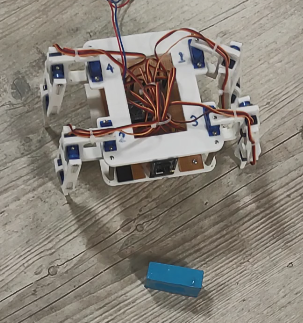
\includegraphics[width=0.4\textwidth]{./images/Chapter5/BlueBackUpview}	
	\caption[-نمای بالا از ربات تشخیص رنگ آبی]{تشخیص رنگ آبی- نمای بالا از ربات}
	\label{تشخیص رنگ آبی}
\end{figure}
\noindent
\unskip

\newpage
\subsection{نتایج مکان‌یابی}

\begin{figure}[H]
	\centering
	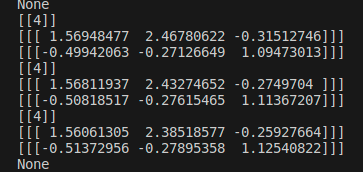
\includegraphics[width=0.6\textwidth]{./images/Chapter5/arucoMatrices}	
	\caption[ زوایا و فواصل از تگ]{زوایا و فواصل از تگ}
	\label{مکان‌یابی}
\end{figure}
\noindent
\unskip

\section{پیشنهادات}
در اين قســمت با توجه به كارهای انجام شــده در اين پژوهش و نتايج حاصــل شــده، پيشــنهاداتی برای كارهای آينده، به شرح زير ارائه مي‌گردد:
\begin{itemize}
	\item
	تست
	\item
	
	\item
	
\end{itemize}